%%%%%%%%%%%%%%%%%%%%%%%%%%%%%%%%%%%%%%%%%%%%%%%%%%%%%%%%%%%%%%
%%%%
%%%%  Project October
%%%%
%%%%%%%%%%%%%%%%%%%%%%%%%%%%%%%%%%%%%%%%%%%%%%%%%%%%%%%%%%%%%%
\documentclass[11pt,letterpaper]{article}
\usepackage[utf8]{inputenc}
\usepackage[letterpaper,includeheadfoot, top=0.5cm, bottom=3.0cm, right=2.0cm, left=2.0cm]{geometry}
\renewcommand{\familydefault}{\sfdefault}

\usepackage{graphicx}
\usepackage{color}
\usepackage{amsmath}
\usepackage{fancyhdr}
\usepackage{paralist}
\usepackage{hyperref}
\usepackage{subfig}
\usepackage{pdfpages}
\usepackage{amssymb}
\usepackage{url}
\usepackage{listings}

\usepackage{listings} %Code
\lstset{language=C, tabsize=4,framexleftmargin=5mm,breaklines=true}

\hypersetup{
    colorlinks,%
    citecolor=black,%
    filecolor=black,%
    linkcolor=black,%
    urlcolor=black
}

\begin{document}
%\begin{sf}

\newpage
\pagestyle{fancy}
\fancyhf{}
\fancyhead[L]{ 
\includegraphics[scale=0.3]{img/cwru-formal-logo-blue-no-tag.png} }
\vspace*{6cm}
\begin{center}
\Huge  {Project October}\\
\vspace{1cm}
\huge {Read news that you want to read}\\
\vspace{1cm}
\end{center}
%----------------- Names ------------------------
\vfill
\begin{flushright}
\begin{tabular}{ll}
Authors: & Rajesh Cherukuri, Tom Dooner, Mika Little, Brian Stack\\
Project: & Project October\\
Date: & \today
\end{tabular}
\end{flushright}

\newpage
\pagestyle{fancy}
\fancyhf{}

%\fancyhead[L]{\rightmark}
\fancyhead[L]{\small \rm \textit{\rightmark}}
\fancyhead[R]{\small \rm \textbf{\thepage}}


%\fancyfoot[L]{\small \rm \textit{Pie de página - Izquierda}}
%\fancyfoot[R]{\small \rm \textit{Pie de página - Derecha}}
%\fancyfoot[C]{\thepage} %Centro

\renewcommand{\sectionmark}[1]{\markright{\thesection.\ #1}}
\renewcommand{\headrulewidth}{0.5pt}
\renewcommand{\footrulewidth}{0.5pt}

% =============== Index ===============

\tableofcontents
\listoffigures

% =============== Section ===============
\newpage
\section{Abstract}

In modern news aggregation services, such as Reddit, Slashdot, Digg, and Hacker News, longtime members report noticing a marked decrease in quality of discourse as the services gain mainstream attention.
This gradual but irreversible decline heralds back to the newsgroup era, when new college students would log in for the first time come September, causing an influx of new users and subsequently diluting discussion upon the sites which they joined.
As an example, after AOL opened newsgroups to the masses, the community standards continued to
devolve, according to newsgroup veterans\cite{september}. This gradual decline of content quality due to
large numbers of new users came to be known as ``Eternal September'', being ``Eternal'' as nowadays,
the influx of new users is no longer restricted to September, but now persists through all months of the year.

The inevitable loss of the longtime members further perpetuates the problem, and causes large numbers of excellent contributors to feel out-of-place in their own community.
We aim to engineer a service that uses technological principles to avoid this, thus improving the user experience and allowing a large community to benefit from thoughtful discourse and interesting articles. \\

\newpage

%----Everything else----%

\section{Project October: Hybrid Recommender System}

Due to the ever-growing amount of information available online, the need for a highly developed personalization and filtering system is growing significantly.
Recommender systems constitute a specific type of information filtering that
attempt to present items according the interests expressed by a user\cite{adom}.
Most web recommenders are employed for e-commerce applications or customer
adapted websites, which assist users in decision making by providing
personalized information \cite{linden}, but the same techniques that
suggest related items on e-commerce websites can recommend news articles to users as well.
We believe Project October is the first attempt to apply recommendation techniques to social news aggregation.

\subsection{Background}
It is our hypothesis that the recommendation of news sources will provide a scalable community experience that can be tailored to each person's interests.
Providing an automatic, customized, recommendation of articles will prevent the community from being diluted by new users and thus prevent the Eternal September phenomenon.
Each user will have their own viewing environment curated for them, with different mindsets and preferences forming their own communities in which like-minded individuals can partake in discussion, eliminating the cross-contamination of user bases.

This proposal discusses an implementation of a hybrid collaborative and content-based filtering approach for a web-based recommender system (``October'').
In particular, we will be linking various news sources and user submitted sources.
The resulting network of user-item relations and associated content features is converted into a unified mathematical model, which is applicable to our underlying neighbor-based prediction algorithm.
By means of various experiments, we demonstrate the influence of supplementary users as well as item features on the prediction accuracy of October, our proposed hybrid recommender. In order to decrease system runtime and to reveal latent user and item relations, we factorize our hybrid model via singular value decomposition (SVD).

For the development and evaluation of our proposed hybrid recommender system, we make use of various news outlets and user recommendations, importing them into a graph database.
Both corpora are joined in a unified mathematical model, which describes the complex network of interdependencies.

\section{Application}
\subsection{Frontend}
The frontend will be a standard social news aggregator.
Upon going to the homepage, new and logged-out users will be presented with a splash page that describes the nature of Project October and offers a registration link.
Users can register for the application by selecting a username and password.

When logged in, users will be presented with their personalized content.
The design is modelled after the front page of a newspaper -- articles that are evaluated to be more interesting to a user will be placed in more prominent positions while articles that are deemed less relevant to the user's interest will fill the side columns, be located further down the page, and occupy less space.
Users will be able to click on the headline (or associated image, if existent) to be taken to the original news source.

Each news article will feature a link to view the associated comments as well as an icon (located in the corner of the article text/image) displaying the credibility (``cred'') a given article possesses.
This is analogous to upvoting in Reddit, except that giving an article cred on October will inform the recommendation engine of your individual preference, rather than directly impacting the weighting of an article by a predefined formula. Therefore, cred serves two purposes: 1. To inform other users of the quality of the article. 2. To inform the recommender system of the user's interests. 

\subsubsection{Backend}
% Tom: The backend will use a graph database, yadda yadda
% Raja: Hey! The backend does more than that!!
% Tom: zzzzzzzzzzzzzzzz

The backend will contain a recommender system, which will consist of a text
classifier for incoming \& existing articles to be indexed into a graph
database, a learning algorithm to combine what the recommender has learned about
the user with the index information, and finally an API to receive queries and
return results. The text classifier will be a combination of Latent Semantic
Analysis with Singular Value Decomposition and Latent Dirchlet Allocation
\cite{lda}, allowing for the clustering of learned topics to create categories
of topics while maintaining coherence to produce an index similar to that formed
by human judgement. As for the learning algorithm, we will be using a custom
bayesian framework \cite{bayesian} that will allow for weighting based on a particular user's current interest instead of a stored calculated interest or utilizing the general population's interests.
Finally, the method of receiving queries and returning results will utilize an API, which is discussed in the following section.

Essentially the approach works as follows:
    \begin{enumerate}
        \item October predicts the user’s authentic news interests regardless of the news trend, using the user’s clicks in each past time period
        \item Predictions made with data in a series of past time periods are combined to gain an accurate prediction of the user’s authentic news interests
        \item October predicts the user’s current interests by combining their authentic news interests and the current news trend in the cluster the user belongs to within the property graph.
    \end{enumerate}

\subsubsection{Frontend/Backend API}
\label{sec:api}
October will employ an API to promote separation between the frontend and the backend recommender system.
This will provide a clear interface and facilitate easy simultaneous development of both parts of October.

To implement the API, we will use Apache Thrift, an Interface Description Language\cite{thrift}.
The essence of the API is simple, featuring primarily two types of calls:
\begin{description}
\item[Give recommendations for user $n$]
This is the main output from the backend, returning recommended news stories or comments for a given user.
Ancillary parameters will be added to this to facilitate the frontend placement of articles, e.g. the recommendation confidence and individual article weightings.
\item[User took action $n$]
This is the main input to the backend, allowing it to adjust recommendations according to user action.
The parameters to this API call can be of many types. For example, "User commented on article \#$n$", "User gave cred to comment \#$n$", and "User visited link \#$n$" are all valid parameters for this API call.
\end{description}

These two calls manifest themselves in Thrift with a few simple object
definitions and an interface.  The abbreviated version \texttt{0.1.0} is
attached as Appendix~\ref{app:thrift}.

\section{Methodology}
\subsection{Frontend}
The frontend of the application is written using the \textit{Ruby on Rails} (``Rails'') framework.
Rails employs a Model-View-Controller architecture that allows for easy creation of sites which employ RESTful architecture.
October's Frontend will maintain collections of objects (such as Posts, Comments, Users, etc., see the database diagram in Figure \ref{fig:database}), and allow operations on those objects, so it is a natural fit for a framework such as Rails.
Through the use of the bundled Object Relational Mapper \textit{ActiveRecord}, common database queries will be abstracted away from the frontend.

We use HAML as an HTML templating engine, as its indent-based structure allows for an expressive and concise representation of HTML.
Other frontend technologies we employ include SASS as a templating language for CSS, and CoffeeScript, which compiles to JavaScript.
The management of all static assets is handled automatically by the Rails Asset Pipeline, which automatically compiles and minimizes all static assets on every deploy to ensure bandwidth efficiency and, consequently, minimize page load times.

The frontend will collect data from the backend via a Ruby implementation of the Thrift Interface Description Language (see Section \ref{sec:api}) and be responsible for all aspects of displaying that information to the user.

\subsection{Backend}
The backend of the application is written primarily in Scala and utilizes its uniques features for express purposes, such that this language choice is not trivial. The use of Scala was mainly to create potentially high volume services that form distributed systems. As such Scala emphasizes scalability, is a functional language as well as object oriented, statically typed, and best of all works within the Java Virtual Machine. These features allow us to build efficient applications and use the features of the JVM to scale our finished product. Beyond this, while frameworks like Play! were available for use, we chose to develop our project using pure Scala.

As such, the backend is split into 4 components, a classifier, a clusterer, a graph database and a recommender. Titan DB was selected as the graph database service. Titan can allow for supporting thousands of concurrent users reading and writing to a single massive-scale graph. The way we approached using this technology appropriately was to create a property graph structure of our data that was epimorphic to the schema for the frontend database (\ref{fig:backend-graph}). For example, when a user reads an article, a 'read' edge connects the user to the article they have accessed. Moreover, all of the friends of that user now have a connection to that article and may even read it themselves. Essentially, for this property, time can be declared as a primary key. Titan supports vertex-centric indices which ensure $O(log(n))$ lookups of adjacent vertices based on the incident edge labels and properties, where $n$ is the number of edges emanating from the vertex. This ensures that despite the size of the graph, the lookups will not be expensive.

While we can create vertices for users, posts, and comments, etc., for recommendations to be made we require the creation of edges. These edges are implemented to support either user provided information or content-based analysis. As such, we needed to approach how to connect vertices that do not have an explicit relationship. It was determined that in the case of posts, clustering based on topic and sentiment was ideal. We determined that using a naive bayesian classifier to determine the topics of posts and using opinion mining to determine the sentiment was the ideal route. Naive Bayesian classifiers provide the advantage that only a small amount of training data is required to start classification, which is ideal to create relations between posts quickly. Opinion mining was implemented using a knowledge-base, specifically SentiWordNet to extract the semantic and affective information.

Using the information from the related post, comments are connected to posts via a parent edge. This also allows comments to inherit a topic. Unlike Posts, Comments do not undergo opinion mining. In this case, material is too short and at times the semantic meaning of the statement is not always understood. To avoid this pollution, users may tag comments. Initially, users can create these tags on their own, which will undergo a much lighter version of opinion mining. The aggregate of opinions will be kept as a property on the comment's vertex. The reasoning for this lies with the recommendation service.

The recommendation service is the heart of the backend. Though there is some implied complexity with this tool, it is in fact a highly optimized graph traversal tool. The reason for why we can do this is that the requisite edges have been determined so that we simply implement an informed search pattern. As mentioned before, we have grouped posts and comments by topic and sentiment. During this time, we have also grouped these objects under a key and now we intend to apply some function to those groupings. The obvious choice was to utilize the MapReduce pattern. Essentially:
\begin{enumerate}
    \item key: for the incoming object generate a key to group it by
	\item value: before storing the object under the key, process it to yield the value to be stored
	\item reduce: when the stream is empty, apply this function to all the values stored at each key.
\end{enumerate} 
Since we specified Titan provides the groupings in $O(log(n))$ time, the concern is the amount of space required to execute our intended traversals which comes to $O(log(n))$ traversals, where $n$ is the size of the largest cluster.

Overall, we expected the recommender and its associated services to have a high time and space complexity. This was not the case; In fact, initial performance tests can be seen in \ref{fig:test-performance}. The yellow represents a user with only the initial training connections, green represents a user with expanded number of connections but no connections to other users still, and the blue represents a user with expanded connections and connections to other users. The y-axis is the response time and the x-axis is the number of nodes in the graph. To show any noticeable change, it required showing the scale at .2-.7 milliseconds. 


% TODO: Write some more here...
% "This section should discuss any data structure design/maintenance problems,
% or algorithmic problems / challenges, and how they will be/are solved; time
% and space complexity analysis (if needed) of your algorithms, etc."

\subsection{Project Management}
We will manage the project using agile development methodologies with a focus on progressive elaboration and documentation for the purposes of this project.

\subsubsection{Agile Development}
In order to stay within the bounds of Agile Development while still maintaining the requisite documentation, we will be creating documentation at the end of each release.
In order to schedule work, we have employed Pivotal Tracker, an online task management solution.
From the queue, we will assign tasks as we finish previous tasks.
The work naturally fits into two main categories -- frontend and backend.
Work relating to each category will be assigned to the same people until we make enough progress to cross between teams at will.
At least until that point, Brian and Rajesh will work on the backend while Tom and Mika create the frontend.

\subsubsection{Scrum}
We will meet every Monday, Wednesday, and Friday at 3:55pm to have a short meeting to discuss the current progress, any stumbling blocks, and what work is coming up in the immediate future.

\subsubsection{Release Schedule}
Releases are bi-weekly and will include a team review as well as planning for the next release.
Release dates will involve pushing the current state of the project to a continuous integration service (http://travis-ci.org), after which automated deployment will be executed.

\subsubsection{Iterations}
We plan to have weekly iterations.
At the end of each iteration, team members will re-sync and make sure that we have a clear outline for the next iteration.

\section{Software Design}
% This section will describe the progress towards the usual software design information, with likely components on
% - Application Software Requirements
% - Application Software Specifications
% - Software Architecture (i.e., client - server architecture; three - tiered design, etc.)
% - Design Document

\subsection{Intended Audience}
We intend Project October to be open to the public.
At launch, we expect the user base to be somewhat technical in nature, being some of the Internet's power users, however, October should support the registration of any internet user.

\subsection{Homepage Requirements}
The are two cases for the homepage: logged in users and logged out users.

Logged out users should arrive at the homepage and be presented with a splash page of sample content and a description of October's features.
There should be a registration link so that interested users can register for their own account.

Logged in users should, upon landing on the homepage, be presented with a display of news articles.
The display will be pictures (when available) along with the headlines for each article.
Each article should be accompanied with links to positively influence the article's recommendation rank, to negatively influence the article, and to comment on the article.

\subsection{User Creation/Login/Display Requirements}
Internet travelers should be able to create accounts on October easily by providing minimal information -- simply their desired username, their email, and a password.
After creating a user, an email should be sent to the user welcoming them to October and containing a confirmation link to confirm their email address.

When a user first uses October, we don't know anything about that user's interests. Users should be shown various sample topics until the recommender is confident enough in their browsing habits to hazard a recommendation.

Every mention of a user's name (i.e. the credit for who posted an article or comment) should be a link to a user profile page. This profile page will have a list of the user's comments and post submitting history.

\subsection{Article Posting Requirements}
Logged in users should be able to click a prominent link on the homepage to submit a story.
The submit story page will ask for the link to the desired story, and show the results of scraping that story's contents (see Section \ref{sec:scraping} for more about scraping).
If all looks good to the user, he or she can click a ``Post!'' button, which will persist the news story in all appropriate databases.

\subsection{User Profile Page Requirements}
\subsection{Article Page Requirements}
\subsection{Frontend $\leftrightarrow$ Backend API Requirements}
\subsection{Web Scraping Requirements}
\label{sec:scraping}
When a user submits a link to a news article, October needs to know more about that article than its URL: the title of the article, any associated images, as well as the article's full text (for analysis purposes).
We will employ a library which, given the URL to a webpage, will perform calculations and extract the main text of the article as well as make recommendations on what image might be the most relevant image on the page.
The requirements of the web scraper are intended to allow the backend's NLP functionality to process the raw text of the article easily. It executes in three phases:
\begin{enumerate}
  \item Document Cleaning
  \item Content Extraction
  \item Document Cleanup
\end{enumerate}
Ultimately, this entails cleaning out junk and comments, grab the cluster of relevant text, attempt to determine the best image, and return these. Specifically the image extraction was troublesome, as Java's image functions were completely unreliable, which was resolved by using ImageMagick.

\subsection{Backend Requirements} % Expand into multiple sections?

\section{Project Management--Administrative Details}
% Design/update your Gantt chart to show any changes in milestones, timetable,
% or responsibility (especially if there are multiple team members). Be sure to
% properly indicate who is actually performing each task and the degree of
% completion of each task.  Describe how well the project management plan is
% working. Were there unforeseen problems with any of the tasks that you ha ve
% had to work around? Are there delays in obtaining parts or software?  Were
% major changes to the management plan or back - up plans requ ired and
% implemented? What work - arounds were necessary to keep the project on
% schedule?  It is very important that you des cribe any changes in the project
% plan since the proposal and the reasons for them.  Finally, use your
% management plan to carefully think about what can be realistically done by
% your 3 team between now and the end of the semester.

\section{User Interface}
% This section contains the user interface of the application. It should have
% numbered figures with titles and screenshots of the GUI components, as well
% as explanations.


\section{Testing \& Evaluation}
% This section should discuss any testing and evaluation done so far.

\section{Project Progress}
% This section should summarize the progress (or the lack of it) so far, and
% address any issues that have arisen recently.

\subsection{Discussions \& Conclusions}
% These conclusions are not really conclusions since your project is not yet
% finished. In this section you should discuss whether the project is on
% schedule for completion at the end of the semester. Are there major problems
% which require a reevaluation of the project results? If not, what is the new
% schedule and what do you plan to have done by the end of the semester? You
% can also comment on things which have worked better than expected or proved
% easier to solve.

\section{Appendix}

% ============= References ==============
\newpage
\newpage
\begin{thebibliography}{6}
  \bibitem{adom} Gediminas Adomavicius , Alexander Tuzhilin, \textit{Toward the Next Generation of Recommender Systems: A Survey of the State-of-the-Art and Possible Extensions}, IEEE Transactions on Knowledge and Data Engineering, v.17 n.6, p.734-749, June 2005  [doi>10.1109/TKDE.2005.99]

  \bibitem{linden} Greg Linden , Brent Smith , Jeremy York, \textit{Amazon.com Recommendations: Item-to-Item Collaborative Filtering}, IEEE Internet Computing, v.7 n.1, p.76-80, January 2003  [doi>10.1109/MIC.2003.1167344]

  \bibitem{bayesian} Jensen, V. \textit{Bayesian Networks and Decision Graphs}. Springer, 2001

  \bibitem{lda} Arthur Asuncion, Padhraic Smyth, Max Welling. \textit{Asynchronous Distributed Learning of Topic Models}. NIPS 2008.

  \bibitem{september} \url{http://en.wikipedia.org/wiki/Eternal\_September}

  \bibitem{thrift} \url{http://en.wikipedia.org/wiki/Apache\_Thrift}

\end{thebibliography}

% ============= Database Schematic ==============
\begin{figure}
\centering
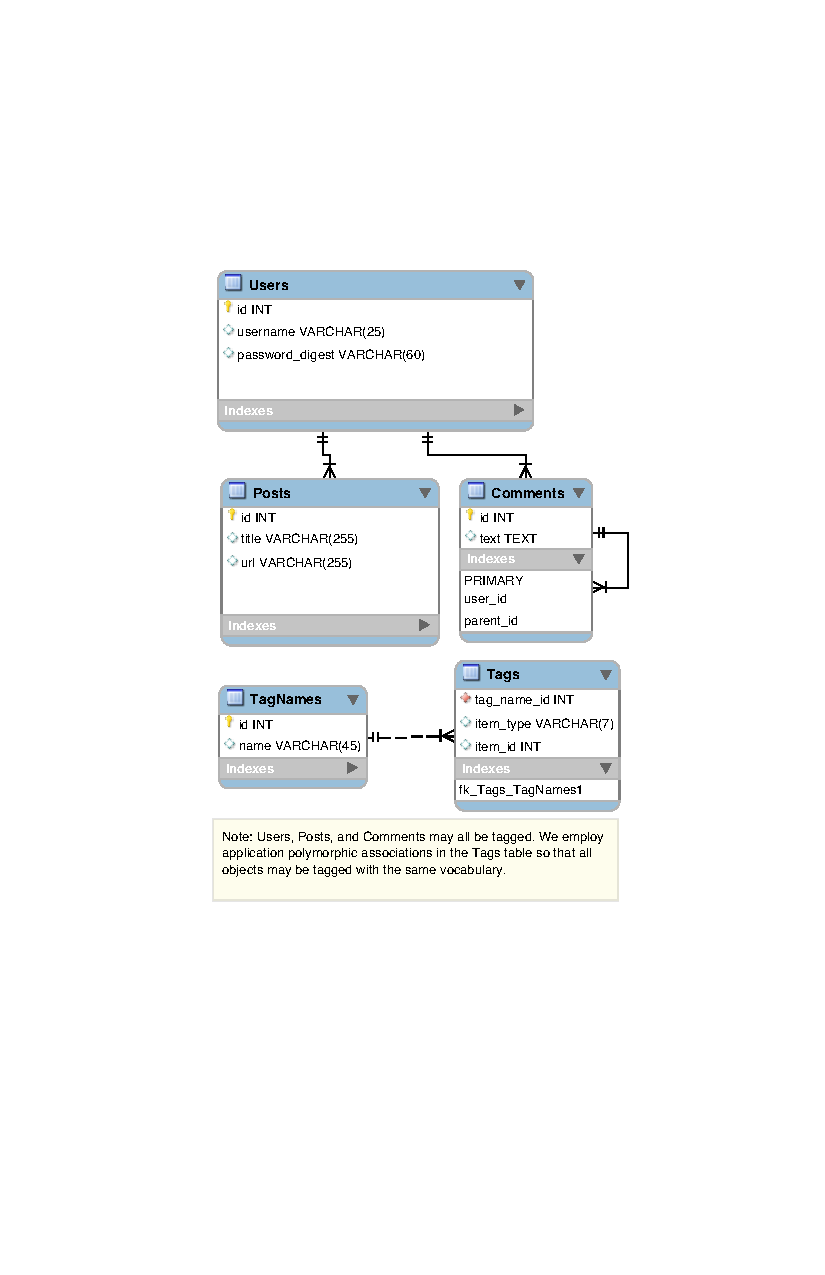
\includegraphics{img/db_diagram.pdf}
\caption{Frontend Database Relational Diagram}
\label{fig:database}
\end{figure}

\begin{figure}
\centering
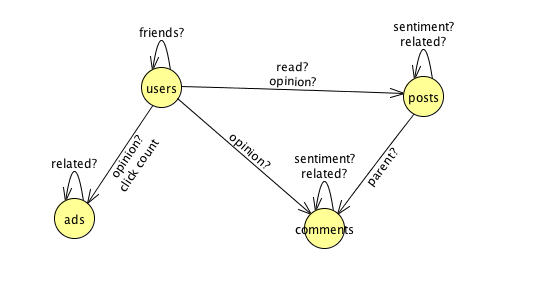
\includegraphics{img/recsys_model.svg}
\caption{Backend Database Model}
\label{fig:backend-graph}
\end{figure}

\newpage
\appendix
\section{Thrift API Definition}
\label{app:thrift}
\begin{verbatim}
#
# Structs
#

/** A single post with its calculated weight.
 * @param post_id, the unique id of a post.
 * @param weight, the "importance" of the post to the querying user [0,1].
 */
struct Post {
    1: required i64 post_id,
    2: optional double weight,
}

/** A list of posts along with a confidence for the accuracy of the list.
 * @param confidence, the confidence in the results.
 * @param posts, a list of Posts.
 */
struct PostList {
    1: optional double confidence,
    2: required list<Post> posts,
}

/** The types of actions that can be performed in a triple (subject, verb, object) */
enum Action {
    READ,
    VOTE_UP,
    VOTE_DOWN,
    VOTE_NEGATE,
    POST,
    COMMENT,
    REPORT,
    TAG
}

#
# Exceptions
#

/** The queried object does not exist. */
exception NotFoundException {
}

/** There was an error processing the request */
exception EngineException {
    1: required string why,
}

/** Request took too long to process */
exception TimeoutException {
}

#
# Service
#

service Recommender {

    /** Test for connectivity */
    string ping() throws (1: TimeoutException te),

    /** Request a list of posts that are most appropriate for a user
     * @param user_id, the user that the posts are being requested for
     */
    PostList recPosts(1: required i64 user_id) throws (1: NotFoundException nfe, 2: EngineException ee, 3: TimeoutException te),

    /** Alert the recommender that a user has actioned a post
     * @param user_id, the user that performed the action
     * @param verb, the action taken (this is from the Action enum)
     * @param post_id, the post that the action is being performed on
     */
    void user_v_post(1: required i64 user_id, 2: required Action verb, 3: required i64 post_id) throws (1: NotFoundException nfe),

    /** Alert the recommender that a user has actioned a comment
     * @param user_id, the user that performed the action
     * @param verb, the action taken (this is from the Action enum)
     * @param comment_id, the comment that the action is being performed on
     */
    void user_v_comment(1: required i64 user_id, 2: required Action verb, 3: required i64 comment_id) throws (1: NotFoundException nfe),
}
\end{verbatim}
\section{Figures}
\begin{figure}
\centering
\includegraphics{img/recsys_performance.png}
\caption{Backend Performance Graph}
\label{fig:test-performance}
\end{figure}



\section{Database Design}
\subsection{Frontend Database}
\subsection{Backend Database}

\section{User Manual}

\section{Programmers Manual}
% ============= FIN ==============

\end{document}
